\subsection{Torque requirements}
The key outcome for single primitive optimisation is to produce physically realisable and useful constraints while minimising the required torque. It is therefore necessary to review the torque requirements and state evolution of the optimised constraints using the simulator described in Chapter \ref{chap:sim}, especially noting that the torque is only optimised for a particular initial velocity. In order to retain clarity, results in this section are limited to the 2-link compass-gait walker such that there is only a single torque.

The torque required for a particular virtual constraint to be completed with a range of initial velocities is presented in Figure \ref{fig:singleflattorque}. The result is quite predictable; the torque curves all have reasonably similar shapes (ignoring some numerical noise), with the footsteps with higher initial velocities requiring more torque and finishing earlier than those which started more slowly. This has the effect of contracting the curve in time but expanding it in the torque dimension. Since the shape of the torque curve is well behaved in its dependence on velocity, it is reasonable to expect near-optimality for initial velocities near the nominal.

\begin{figure}
\centering
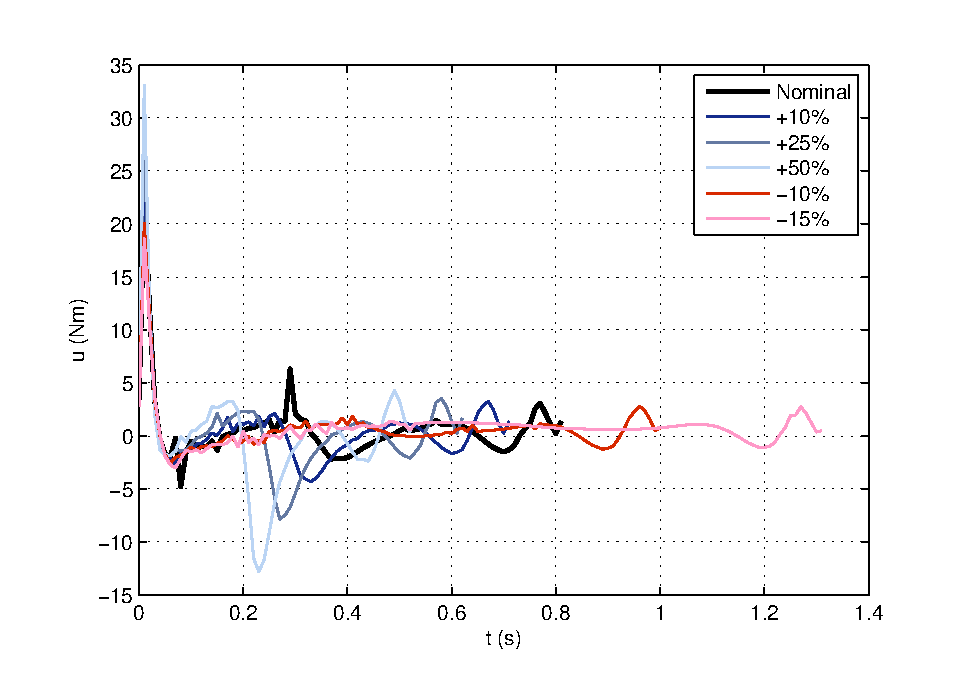
\includegraphics[width=0.8\linewidth]{7Results/singleflattorque}
\caption[Torque curves for differing initial velocities on flat ground]{Torque curves for different initial velocities of a virtual constraint on flat ground with $s_l=0.3$m}
\label{fig:singleflattorque}
\end{figure}

An alternative method for assessing the closeness to optimality of the virtual constraints for non-nominal velocities is to optimise two VCs with the same beginning and final configurations but differing initial velocities and to compare the torque curves. The result of this analysis with one VC optimised using the nominal velocity definition from Section \ref{sec:optmethod} the other with a nominal velocity 20\% larger is displayed in Figure \ref{fig:twonomvels}. From this plot, we observe the sensitivity in the optimisation to the initial velocity; the curves show a much stronger difference than observed in Figure \ref{fig:singleflattorque}. Even so, the curves show a somewhat similar shape; while the optimality of the curve is clearly not maintained across a range of velocities, the torque requirements are well behaved.

\begin{figure}
\centering
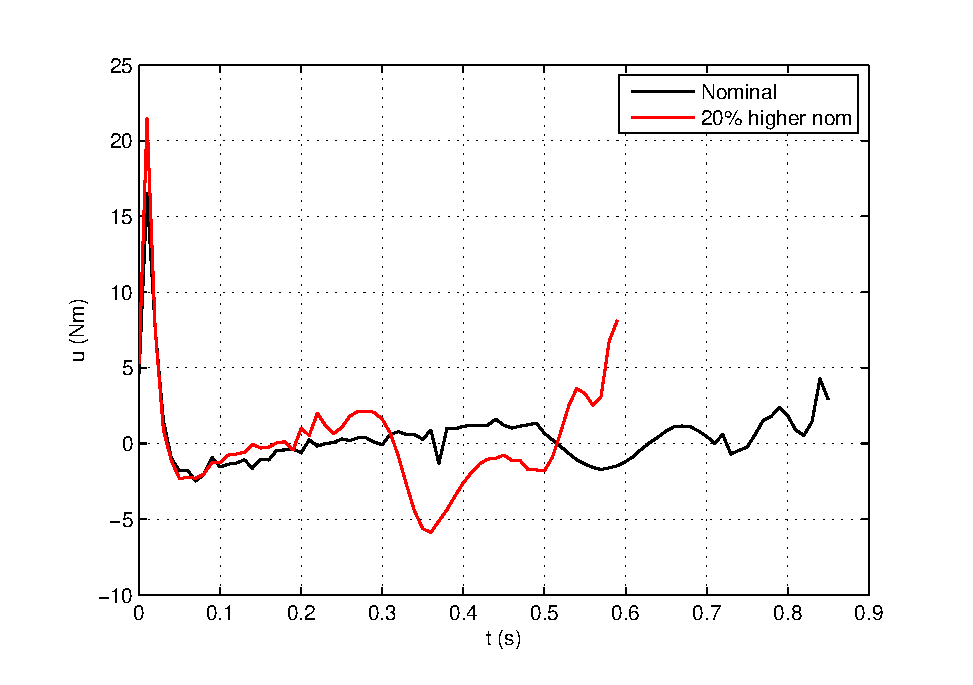
\includegraphics[width=0.8\linewidth]{7Results/twonomvels}
\caption[Torque curves with differing nominal velocities]{Torque curves for similar constraints with the same initial velocity but optimised for different nominal velocities over a single footstep}
\label{fig:twonomvels}
\end{figure}

Note that the torque in these plots seem excessive; from the literature one would expect to see peak torques below 1 Nm \cite{westervelt2007feedback, collins2005efficient}. It is not clear what is causing this; the calculation of nominal torque closely matches that produced by PD control (see Figure \ref{fig:pdmatchesnom}), therefore the simulation is consistent with the model used for production of the virtual constraints. While the torque appears to be significantly higher than it should be, the actual values are not of critical importance, since this is a largely theoretical exercise given the simple model used. A more complete model will include toe-off forces which are likely to lead to significantly smaller hip torques, particularly at the initial point of the constraint, which is where we observe the largest torque.

\begin{figure}
\centering
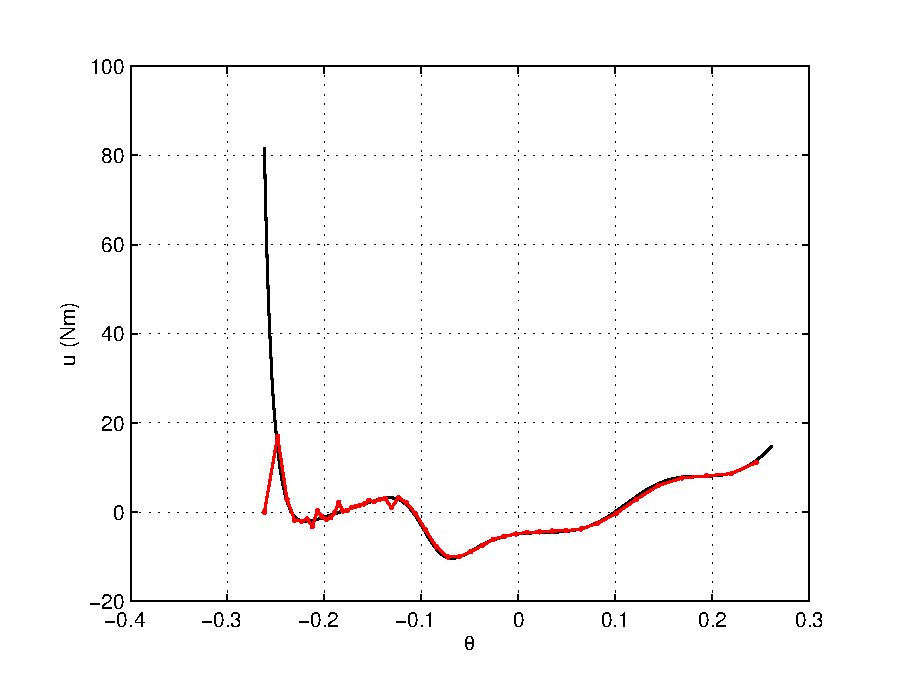
\includegraphics[width=0.8\linewidth]{7Results/pdmatchesnom}
\caption{Nominal torque and simulated PD torque for a single virtual constraint}
\label{fig:pdmatchesnom}
\end{figure}


\subsection{Kinetic energy mutations}
The kinetic energy change over the virtual constraint, like the torque, is dependent on the initial velocity. In principle, this may be computed analytically, however since the analytical solution is dependent on the virtual constraint being perfectly maintained, using a simulator is likely to provide a more realistic expectation of the extent of the dependence of the kinetic energy mutation on the initial velocity. It is important that the desired energy change roughly equals the observed change for a reasonable range of initial velocities, since the richness of the library is dependent on the existence of a range of kinetic energy mutations available at each step for any given initial velocity.

Table \ref{tab:vcenergy} presents the observed kinetic energy changes with varying initial velocities for a set of sample virtual constraints, each with the same initial and final configurations. Empty table cells correspond to the virtual constraint being unable to be completed due to insufficient initial velocity. A somewhat surprising result is how poorly the kinetic energy mutations are met at the nominal velocity. This is due to the numerical inaccuracies in optimising the constraint as well as those introduced in the simulation. Encouragingly, while there is a notable increase in the loss of kinetic energy with increasing velocity, there remains a genuine range in the kinetic energy mutations available independent of the initial velocity.

\begin{table}
	\centering
	\begin{tabular}{ r || c | c | c | c | c | c}
		Nominal & $0.75~\dot{\theta}_{\mathrm{nom}}$ & $0.9~\dot{\theta}_{\mathrm{nom}}$ & $\dot{\theta}_{\mathrm{nom}}$ & $1.1~\dot{\theta}_{\mathrm{nom}}$ & $1.25~\dot{\theta}_{\mathrm{nom}}$ & $1.5~\dot{\theta}_{\mathrm{nom}}$ \\ \hline
		-0.05 & -0.0373 & -0.0494 & -0.0571 & -0.0695 & -0.0792 & -0.1034  \\
		0     & -0.0059 & -0.0162 & -0.0100 & -0.0198 & -0.0309 & -0.0388 \\
		0.05  &    -    &  0.0240 &  0.0096 &  0.0060 &  0.0027 & -0.0206  \\
		0.1   &    -    &    -    &  0.0473 &  0.0369 &  0.0302 &  0.0258
	\end{tabular}
	\caption[Observed kinetic energy mutations with varying initial velocity]{Observed kinetic energy mutations in joules with varying initial velocity}
	\label{tab:vcenergy}
\end{table}

A more concerning result is the apparent difficulty of adding mechanical energy to the robot through the application of hip torque over a footstep. This may be explained by considering that adding energy pushes the robot further from stability. Any errors are magnified and the system, particularly at impact, has considerable tendency toward energy loss. This problem largely originates in the simple model chosen to represent the walkers. An elastic impact model and feet with some appreciable spring force would rectify much of this problem.

\subsection{Varying optimisation parameters}
There are several parameters in the optimisation which can be relatively freely chosen that compromise some aspect of the optimisation result with computational performance. It is important to investigate the effects of varying these parameters such that a good compromise can be achieved for the library generation.

As discussed in Section \ref{sec:numsolacc}, the accuracy of the optimisation is dependent on the grid size. Clearly, a more accurate optimisation is favourable in that the torque is better optimised and the kinetic energy mutation is more accurately set. However,

Additionally, increasing the degree of the Bézier curve enables finer control over the path.

\begin{itemize}
	\item Times to generate using different degrees
	\item and grids
	\item and regularisation constant
\end{itemize}